%% Attention-Aware Study Assistant -- Presentation (KIT sdqbeamer)
%% Requires KIT sdqbeamer template installed locally.
%% Compile (recommended): pdflatex -> biber -> pdflatex -> pdflatex

\documentclass{sdqbeamer}

%% Title image (provided by KIT template)
\titleimage{banner_2020_kit}

%% Group name (optional)
\groupname{GenAI System Building Challenge \textbar{} Lab Hackathon}

\title[Attention-Aware Study Assistant]{Attention-Aware Study Assistant}
\subtitle{An agentic, attention-aware learning system with microservices + GenAI}
\author[Team]{Team Project}\date{May 2026}

\usepackage{booktabs}
\usepackage{tabularx}
\usepackage{array}
\usepackage{graphicx}
\usepackage{listings}
\usepackage{tikz}
\usetikzlibrary{arrows.meta,positioning,fit,shapes.geometric,shapes.misc}

\lstset{
  basicstyle=\ttfamily\small,
  breaklines=true,
  frame=single,
  columns=fullflexible,
  keepspaces=true
}

% MiKTeX listings doesn't always ship with all language definitions enabled.
% Define a lightweight JavaScript language for the code snippet(s) below.
\lstdefinelanguage{JavaScript}{
  morekeywords={const,let,var,function,return,if,else,for,while,break,continue,new,this,true,false,null,undefined,try,catch,finally,throw,await,async},
  sensitive=true,
  morecomment=[l]{//},
  morecomment=[s]{/*}{*/},
  morestring=[b]",
  morestring=[b]',
}

\begin{document}

% Title
\KITtitleframe

% Agenda
\begin{frame}{Agenda}
  \tableofcontents
\end{frame}

\section{Problem \& Idea}

\begin{frame}{Core Idea: Attention-Aware Adaptation}
\begin{itemize}
  \item Learners fatigue during long explanations (text or video) and comprehension drops.
  \item Most tutoring systems deliver static output regardless of attention state.
  \item We deliver \textbf{real-time adaptation} of content \emph{and} learning strategy.
  \item Observe behavioral signals (keystrokes, response time, video interactions).
  \item Infer fatigue label: \texttt{FRESH} $\rightarrow$ \texttt{MODERATE} $\rightarrow$ \texttt{TIRED} $\rightarrow$ \texttt{EXHAUSTED}.
  \item Select best teaching mode (detailed / concise / analogy / quiz).
  \item Close the loop with persistence + profile updates.
\end{itemize}
\end{frame}

\begin{frame}{Agentic Loop (ReAct)}
\centering
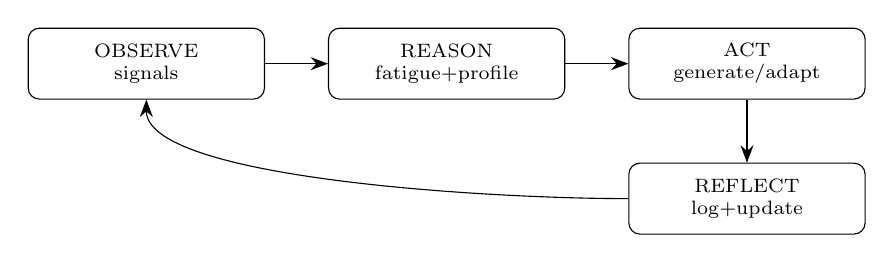
\begin{tikzpicture}[
  node distance=8mm,
  box/.style={draw,rounded corners,align=center,minimum width=30mm,minimum height=9mm,font=\scriptsize},
  arr/.style={-{Stealth[length=2.2mm]}}
]
% Compact 2-row layout (prevents right-side clipping)
\node[box] (obs) {OBSERVE\\signals};
\node[box,right=of obs] (rea) {REASON\\fatigue+profile};
\node[box,right=of rea] (act) {ACT\\generate/adapt};
\node[box,below=of act] (ref) {REFLECT\\log+update};

\draw[arr] (obs) -- (rea);
\draw[arr] (rea) -- (act);
\draw[arr] (act) -- (ref);
\draw[arr] (ref.west) .. controls +(left:18mm) and +(down:10mm) .. (obs.south);
\end{tikzpicture}
\vspace{2mm}

\small The Orchestrator runs this loop on every interaction.
\end{frame}

\section{System Overview}

\begin{frame}{High-Level Architecture (10 Microservices)}
\centering
\vspace{-2mm}
\includegraphics[width=0.95\textwidth,height=0.72\textheight,keepaspectratio]{../image.png}
\end{frame}

\begin{frame}{What Happens on \texttt{/interact}? (Flowchart)}
\centering
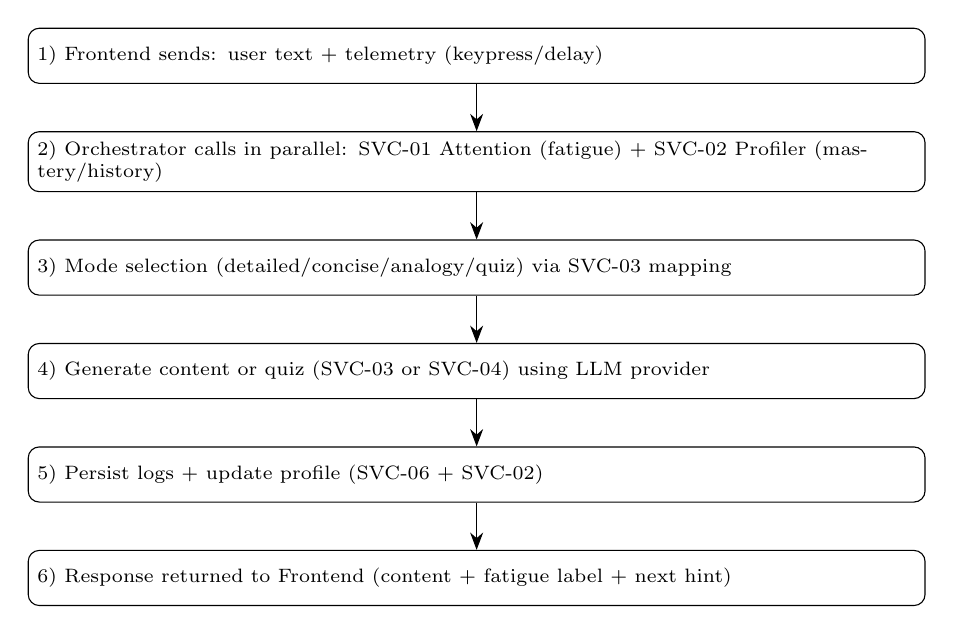
\begin{tikzpicture}[
  node distance=6mm,
  flowstep/.style={draw,rounded corners,align=left,text width=0.92\textwidth,minimum height=7mm,font=\scriptsize},
  arr/.style={-{Stealth[length=2.2mm]}}
]
\node[flowstep] (s1) {1) Frontend sends: user text + telemetry (keypress/delay)};
\node[flowstep,below=of s1] (s2) {2) Orchestrator calls in parallel: SVC-01 Attention (fatigue) + SVC-02 Profiler (mastery/history)};
\node[flowstep,below=of s2] (s3) {3) Mode selection (detailed/concise/analogy/quiz) via SVC-03 mapping};
\node[flowstep,below=of s3] (s4) {4) Generate content or quiz (SVC-03 or SVC-04) using LLM provider};
\node[flowstep,below=of s4] (s5) {5) Persist logs + update profile (SVC-06 + SVC-02)};
\node[flowstep,below=of s5] (s6) {6) Response returned to Frontend (content + fatigue label + next hint)};
\draw[arr] (s1) -- (s2);
\draw[arr] (s2) -- (s3);
\draw[arr] (s3) -- (s4);
\draw[arr] (s4) -- (s5);
\draw[arr] (s5) -- (s6);
\end{tikzpicture}
\end{frame}

\section{Microservices}

\begin{frame}{Microservices at a Glance}
\small
\begin{tabularx}{\textwidth}{@{}l l X@{}}
\toprule
\textbf{ID} & \textbf{Port} & \textbf{Responsibility}\\
\midrule
SVC-01 & 8001 & Attention monitor: fatigue from keystrokes, delay, quiz trend\\
SVC-02 & 8002 & Learner profiler: mastery, difficulty, preferred mode, avg fatigue\\
SVC-03 & 8003 & Content adapter: fatigue$\rightarrow$mode mapping + prompt templating (Jinja2)\\
SVC-04 & 8004 & Quiz engine: generate + evaluate (LLM-as-a-judge)\\
SVC-05 & 8000 & Orchestrator: ReAct loop hub, API gateway routing\\
SVC-06 & 8005 & Data store: sessions, interactions, profiles, quiz, video events\\
SVC-07 & 8501 & Streamlit frontend: learning + quiz UI, gauges, history\\
SVC-08 & 8006 & Video fatigue: score from player events + exponential decay\\
SVC-09 & 8007 & YouTube recommender: topic $\rightarrow$ ranked videos (API/scrape)\\
SVC-10 & 8008 & Transcription summary: transcript fetch (3-tier) + structured summary\\
\bottomrule
\end{tabularx}
\end{frame}

\begin{frame}{Orchestrator: Hub-and-Spoke}
\begin{itemize}
  \item All inter-service communication flows through the Orchestrator.
  \item Enables independent deployability and clean separation of concerns.
  \item Key endpoints:
  \begin{itemize}
    \item \texttt{POST /interact} (text learning + quiz flow)
    \item \texttt{POST /video-interact} (video event telemetry)
    \item \texttt{GET /health} (service health checks)
  \end{itemize}
\end{itemize}
\end{frame}

\begin{frame}{Data Persistence (SVC-06)}
\begin{itemize}
  \item SQLAlchemy ORM over SQLite (dev), designed for Postgres (prod).
  \item Core tables (audit trail + personalization):
\end{itemize}
\vspace{-1mm}
\small
\begin{tabularx}{\textwidth}{@{}l X@{}}
\toprule
\textbf{Table} & \textbf{Purpose}\\
\midrule
\texttt{sessions} & session metadata, topic, start/end\\
\texttt{interactions} & every prompt/response with mode + fatigue\\
\texttt{learner\_profiles} & mastery, difficulty, preferences, avg fatigue\\
\texttt{quiz\_records} & questions, answers, score, feedback\\
\texttt{video\_events} & player events + computed fatigue timeline\\
\bottomrule
\end{tabularx}
\end{frame}

\section{GenAI \& Pipelines}

\begin{frame}{LLM Provider Abstraction}
\begin{itemize}
  \item Single interface: \texttt{generate(system\_prompt, user\_message)}.
  \item Provider priority (auto-detect):
  \begin{itemize}
    \item Gemini API key $\rightarrow$ primary (fast, high-quality)
    \item Ollama local $\rightarrow$ offline mode
    \item Anthropic $\rightarrow$ optional fallback
  \end{itemize}
  \item Keeps microservices provider-agnostic.
\end{itemize}
\end{frame}

\begin{frame}{Pipeline: Content Generation}
\centering
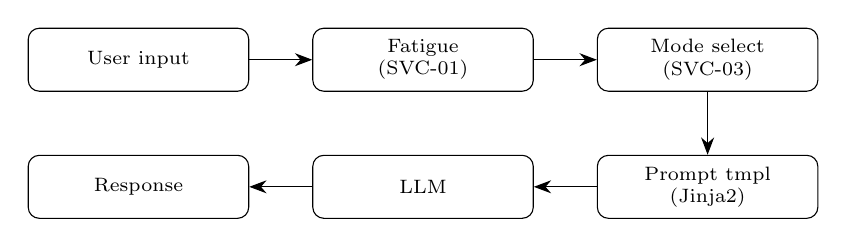
\begin{tikzpicture}[
  node distance=8mm,
  n/.style={draw,rounded corners,align=center,minimum width=28mm,minimum height=8mm,font=\scriptsize},
  arr/.style={-{Stealth[length=2.2mm]}}
]
% Row 1
\node[n] (u) {User input};
\node[n,right=of u] (fat) {Fatigue\\(SVC-01)};
\node[n,right=of fat] (mode) {Mode select\\(SVC-03)};
% Row 2
\node[n,below=of mode] (tmpl) {Prompt tmpl\\(Jinja2)};
\node[n,left=of tmpl] (llm) {LLM};
\node[n,left=of llm] (resp) {Response};

\draw[arr] (u) -- (fat);
\draw[arr] (fat) -- (mode);
\draw[arr] (mode) -- (tmpl);
\draw[arr] (tmpl) -- (llm);
\draw[arr] (llm) -- (resp);
\end{tikzpicture}
\vspace{2mm}

\small Everything is logged to SVC-06 for analytics and replay.
\end{frame}

\begin{frame}{Pipeline: Quiz Generation \& Evaluation}
\centering
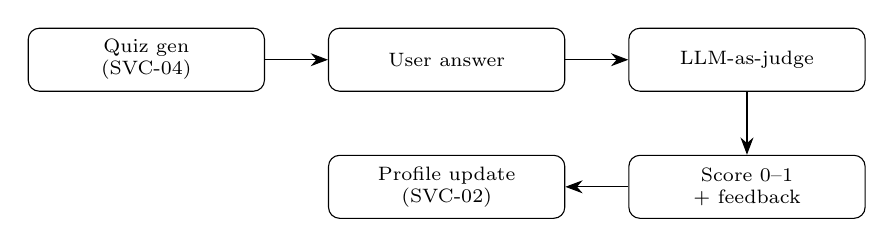
\begin{tikzpicture}[
  node distance=8mm,
  n/.style={draw,rounded corners,align=center,minimum width=30mm,minimum height=8mm,font=\scriptsize},
  arr/.style={-{Stealth[length=2.2mm]}}
]
% Row 1
\node[n] (q) {Quiz gen\\(SVC-04)};
\node[n,right=of q] (ui) {User answer};
\node[n,right=of ui] (judge) {LLM-as-judge};
% Row 2
\node[n,below=of judge] (score) {Score 0--1\\+ feedback};
\node[n,left=of score] (prof) {Profile update\\(SVC-02)};

\draw[arr] (q) -- (ui);
\draw[arr] (ui) -- (judge);
\draw[arr] (judge) -- (score);
\draw[arr] (score) -- (prof);
\end{tikzpicture}
\end{frame}

\begin{frame}{Pipeline: Video Intelligence + Summary Fallback}
\centering
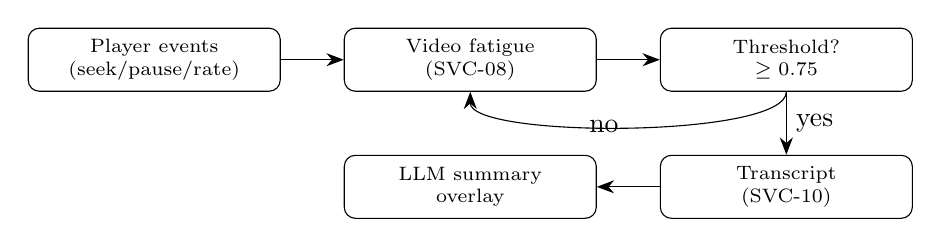
\begin{tikzpicture}[
  node distance=8mm,
  n/.style={draw,rounded corners,align=center,minimum width=32mm,minimum height=8mm,font=\scriptsize},
  arr/.style={-{Stealth[length=2.2mm]}}
]
% Row 1
\node[n] (evt) {Player events\\(seek/pause/rate)};
\node[n,right=of evt] (vf) {Video fatigue\\(SVC-08)};
\node[n,right=of vf] (thr) {Threshold?\\$\ge 0.75$};
% Row 2
\node[n,below=of thr] (tr) {Transcript\\(SVC-10)};
\node[n,left=of tr] (sum) {LLM summary\\overlay};

\draw[arr] (evt) -- (vf);
\draw[arr] (vf) -- (thr);
\draw[arr] (thr) -- node[right]{yes} (tr);
\draw[arr] (tr) -- (sum);
\draw[arr] (thr) .. controls +(down:10mm) and +(down:10mm) .. node[left]{no} (vf);
\end{tikzpicture}
\end{frame}

\section{Fatigue Detection}

\begin{frame}{Fatigue Signals (Text vs Video)}
\small
\begin{tabularx}{\textwidth}{@{}l X X@{}}
\toprule
\textbf{Signal} & \textbf{Text / Quiz Mode} & \textbf{Learning / Video Mode}\\
\midrule
Primary telemetry & Keypress variance + response delay + quiz trend & Seek backward, pauses, speed changes, skips\\
Scoring & Weighted heuristic $\rightarrow$ label & Event impacts + exponential decay\\
Adaptation & Mode switch + quiz trigger & Suggest slowdown / show summary overlay\\
\bottomrule
\end{tabularx}
\vspace{2mm}

\begin{itemize}
  \item Goal: keep cognitive load within a comfortable range.
  \item System reacts before the learner disengages.
\end{itemize}
\end{frame}

\section{Frontend \& UX}

\begin{frame}{Frontend: Learning Mode}
\begin{itemize}
  \item Embedded YouTube player + fatigue gauge (SVG/Plotly).
  \item Buttons: play/pause/seek/speed + one-click explanation.
  \item Local gauge blending (smooth UX) + server sync.
  \item When fatigue crosses threshold: summary overlay replaces remaining video.
\end{itemize}
\end{frame}

\begin{frame}[fragile]{Frontend: Quiz Mode (Telemetry + Feedback)}
\begin{itemize}
  \item Prompt-only interaction with live fatigue gauge in sidebar.
  \item Keypress telemetry captured in-browser and sent with each submission.
  \item Quiz evaluation returns: score, feedback, correct answer + explanation.
\end{itemize}
\vspace{1mm}
\begin{lstlisting}[language=JavaScript]
textarea.addEventListener('keydown', () => {
  timestamps.push(Date.now());
});
// intervals -> SVC-01 for fatigue inference
\end{lstlisting}
\end{frame}

\section{Quality \& Deployment}

\begin{frame}{Testing Strategy}
\begin{itemize}
  \item 8 pytest modules, 30+ tests across key services.
  \item Focus: fatigue scoring correctness, mode mapping, datastore CRUD, pipelines.
  \item Orchestrator integration tests validate full ReAct loop.
\end{itemize}
\end{frame}

\begin{frame}{Cloud-Native Deployment (Concept)}
\centering
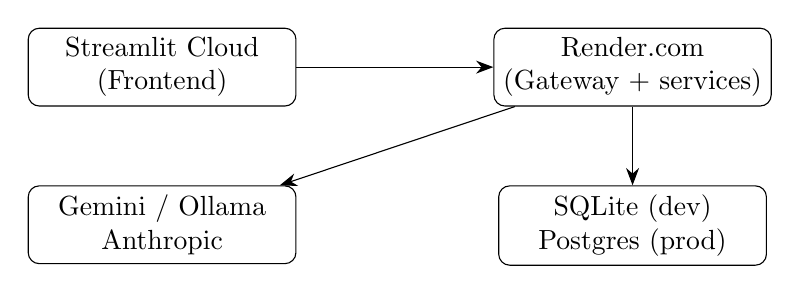
\begin{tikzpicture}[
  node distance=10mm,
  n/.style={draw,rounded corners,align=center,minimum width=34mm,minimum height=9mm},
  arr/.style={-{Stealth[length=2.2mm]}}
]
\node[n] (st) {Streamlit Cloud\\(Frontend)};
\node[n,right=of st,xshift=15mm] (api) {Render.com\\(Gateway + services)};
\node[n,below=of api] (db) {SQLite (dev)\\Postgres (prod)};
\node[n,below=of st] (llm) {Gemini / Ollama\\Anthropic};

\draw[arr] (st) -- (api);
\draw[arr] (api) -- (db);
\draw[arr] (api) -- (llm);
\end{tikzpicture}
\end{frame}

\section{Demo \& Takeaways}

\begin{frame}{Demo Walkthrough (Suggested)}
\begin{enumerate}
  \item Enter a topic and request an explanation (FRESH $\rightarrow$ detailed).
  \item Keep interacting until fatigue rises (mode becomes concise/analogy).
  \item Trigger quiz and show evaluation + profile update.
  \item Switch to video learning; demonstrate backward seeks raising fatigue.
  \item Cross 75\% threshold: show transcript summary overlay.
\end{enumerate}
\end{frame}

\begin{frame}{Conclusion}
\begin{itemize}
  \item A microservices + GenAI system that adapts in real-time to learner fatigue.
  \item ReAct orchestration keeps the architecture modular and testable.
  \item Dual modality: text/quiz adaptation + video intelligence and summary fallback.
\end{itemize}
\vspace{2mm}
\textbf{Next steps (optional):} calibration with real user studies, richer fatigue models, and tighter latency budgets.
\end{frame}

\end{document}
